\section{Theoretical Analysis}
\label{sec:analysis}

In this section, the circuit shown in Figure~\ref{fig:rc} is analysed
theoretically, using both mesh and node analysis.

\section{Mesh Analysis}

The circuit consists of four independent loops, and 11 branches where different currents circulate. These will be our variables in the mesh analysis. The current flow is depicted in Figure ~\ref{fig:current}

\begin{figure}[h] \centering
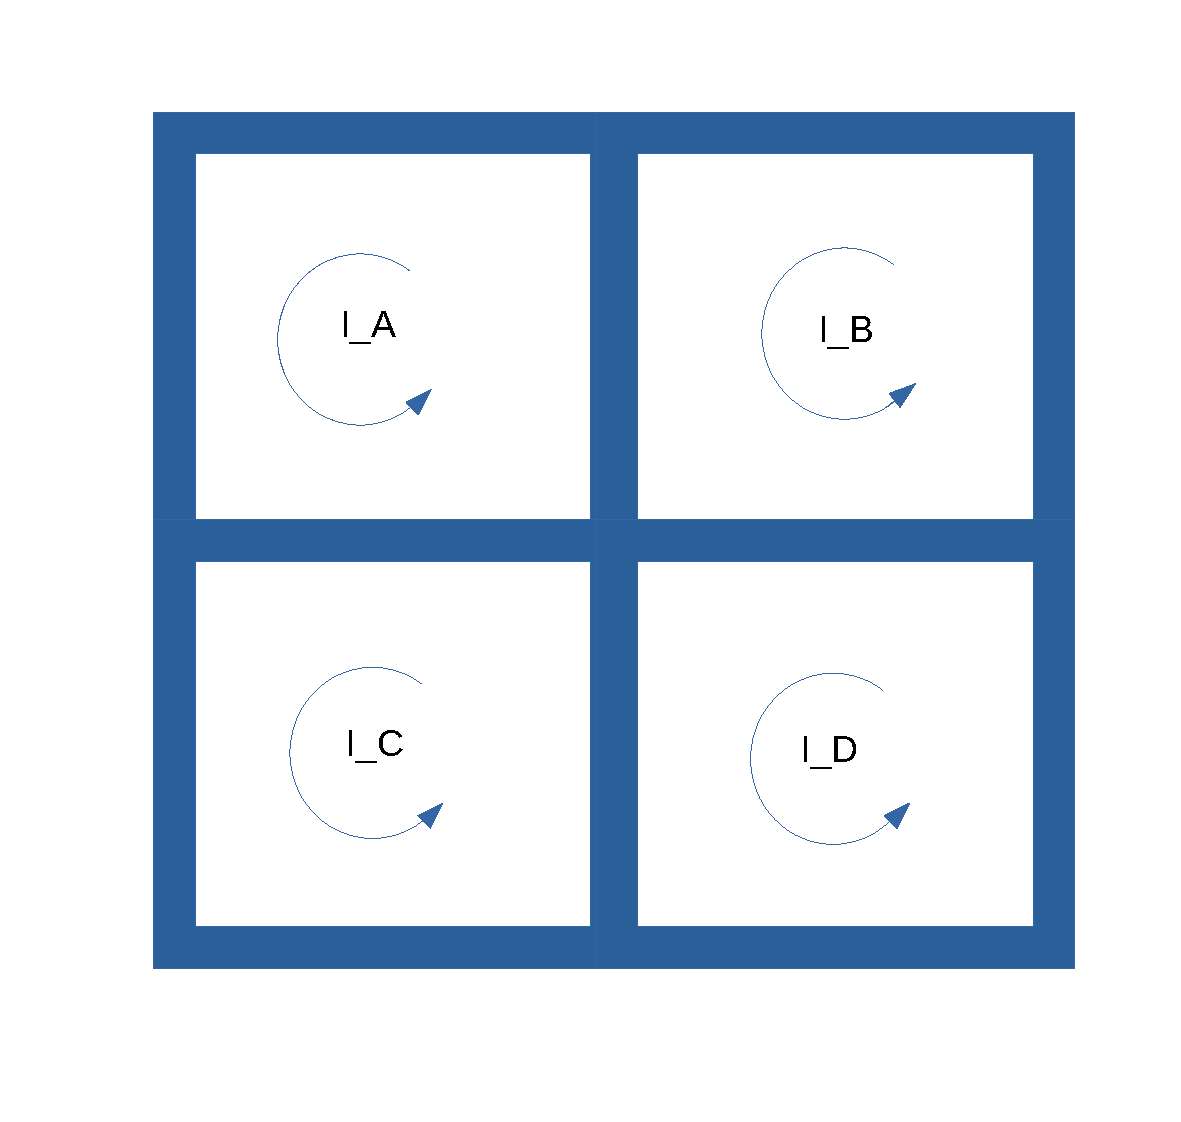
\includegraphics[width=0.4\linewidth]{current.pdf}
\caption{Direction of each mesh current.}
\label{fig:current}
\end{figure}


Applying the Kirchhoff Voltage Law (KVL) in the different loops, we get four different equations which we can then solve as a matrix:
\begin{equation}
  I_D=I;
\end{equation}

\begin{equation}
  (R_1+R_3+R_4)I_A-R_3I_B-R_4I_C=-V_A;
\end{equation}

\begin{equation}
  (R_4+R_6+R_7-K_C)I_C-R_4I_A=0;
\end{equation}

\begin{equation}
  (R_3K_B-1)I_B-R_3K_BI_A=0.
\end{equation}


\begin{equation}
  v_O(t) = v_{On}(t) + v_{Of}(t).
  \label{eq:vo_sol}
\end{equation}

As learned in the theory classes the natural solution is of the form
\begin{equation}
  v_{On}(t) = Ae^{-\frac{t}{RC}},
  \label{eq:vo_nat}
\end{equation}
where $A$ is an integration constant.

\begin{equation}
  V_{Of}(t) = |\bar{V}_{Of}| cos(\omega t + \angle \bar{V}_{Of}),
  \label{eq:vo_for}
\end{equation}


